\section{Application to geophysics} \label{sec:application to geophysics}

We proceed by showcasing the efficacy of our inexact projection framework with a geophysics-inspired application in \emph{data assimilation}. Data assimilation in geophysics involves tracking probability measures for chaotic dynamical systems over time. Traditional Bayesian update methods, such as the continuous-discrete-time feedback particle filter, compute the posterior distribution by propagating particles along an observation flow. Although this method reduces the standard resampling degeneracy, computing continuous log-homotopies (continuous deformations from the prior forecast distribution to the updated posterior distribution) requires solving underdetermined linear partial differential equations, which are prone to numerical ill-conditioning and stiffness~\cite{beeson2024bayesflow}. The optimal transport formulation introduced in this thesis offers an alternative projection mechanism. Rather than integrating a flow formulation to update physical weights, the KR map is learned directly to transport the prior forecast measure onto the analysis posterior. This approach eliminates the need for intermediate numerical integration of the Bayes update flow while preserving the deterministic mapping of state uncertainty.

\subsection{Lorenz 63 model} \label{subsec:lorenz_63}

The mathematical framework for this experiment is based on the stochastic Lorenz 1963 system~\cite{lorenz1963deterministic}. We obtain a dataset of particles for both a prior and posterior distributions from a continuous flow model, which uses coefficients obtained from a truncation of an orthogonal expansion of the Rayleigh-Bénard convection partial differential equations~\cite{beeson2024bayesflow}. To avoid notation ambiguity with the optimal transport unmapped and mapped spatial variables ($x$ and $z$), the three-dimensional ($D=3$) Lorenz state vector is denoted as $q = (q_1, q_2, q_3)^T$. The system evolution is governed by the following stochastic differential equation
\begin{equation*} \label{eq:lorenz_63_sde}
    \mathrm{d}\begin{bmatrix}q_1\\ q_2\\ q_3\end{bmatrix} = \begin{bmatrix}-c_1 & c_1 & 0\\ c_2 & -1 & 0\\ 0 & 0 & -c_3\end{bmatrix}\begin{bmatrix}q_1\\ q_2\\ q_3\end{bmatrix}\mathrm{d}t + \begin{bmatrix}0\\ -q_1 q_3\\ q_1 q_2\end{bmatrix}\mathrm{d}t + \mathrm{d}W_t.
\end{equation*}
Here, $W_t$ represents a standard Brownian motion, which is added as a perturbation to the deterministic Lorenz 1963 (L63) model. This model is popular in geophysics applications, particularly as a low-order model for atmospheric flow. We adopt the standard set of chaotic parameters, with $c_1 = 10$, $c_2 = 28$, and $c_3 = \frac{8}{3}$. This configuration results in a top Lyapunov exponent of $\lambda_1 \approx 0.86$~\cite{beeson2024bayesflow}.

The baseline prior distribution is generated by integrating an initial sample ensemble forward for $0.5$ time units. The initial distribution is Gaussian, with a mean vector of $(1.508870, -1.531271, 25.46091)^T$ and an isotropic standard deviation of $\sqrt{2}$. The discrete-time observation process assumes a full state measurement, represented as $Y_{t_k} = I_{3} q_{t_k} + \xi_{t_k}$, where the measurement noise $\xi_{t_k}$ follows a standard Gaussian distribution $\xi_{t_k} \sim \mathcal{N}(0, I_{3})$.

The reference analysis (posterior) distribution is computed using the continuous-discrete time feedback particle filter evaluated over the observation flow. Figure~\ref{fig:lorenz_63_propagation} shows the projected sample point clouds for the prior and posterior states generated by this baseline method.

\begin{figure}[htbp]
    \centering
    \begin{subfigure}[t]{0.48\textwidth}
        \centering
        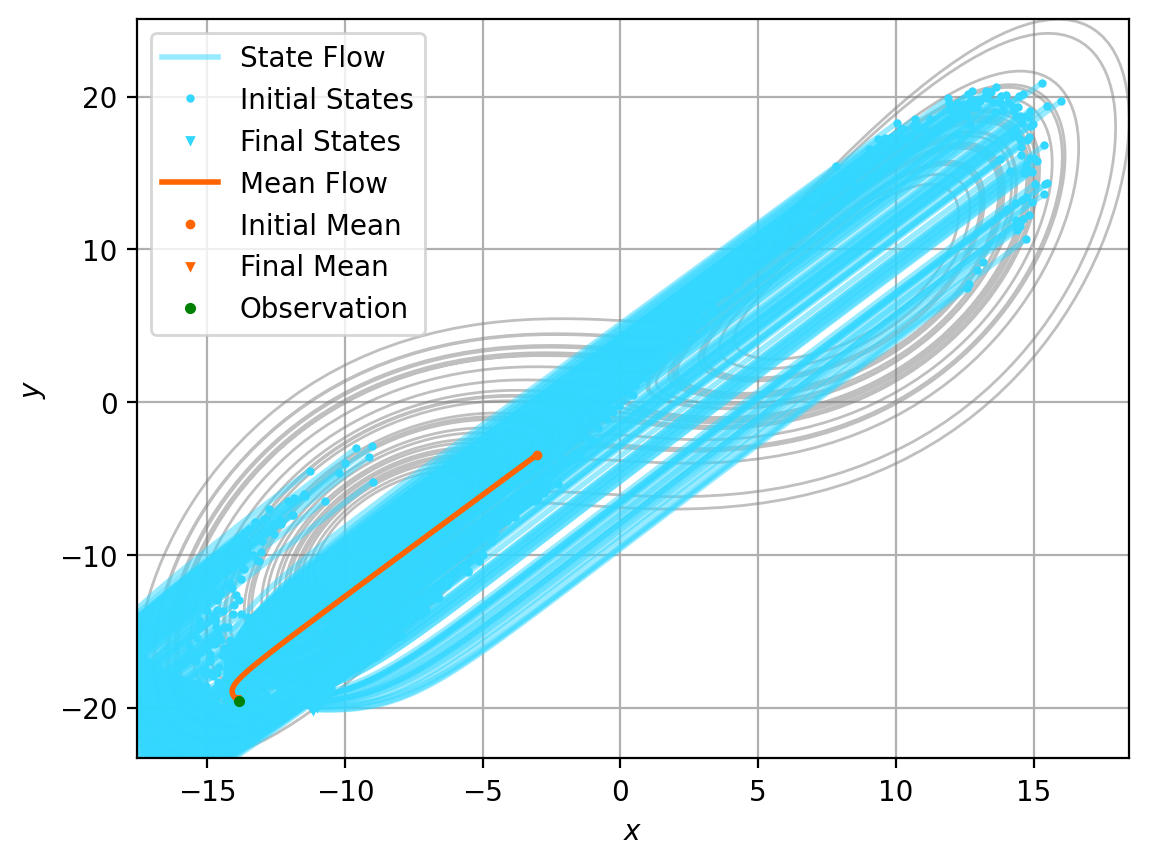
\includegraphics[width=\linewidth]{figures/flow_0_state_0_state_1_signal_background.png}
        \caption{Particle flow in the $q_1$--$q_2$ plane.}
        \label{fig:lorenz_63_propagation_xy}
    \end{subfigure}\hfill
    \begin{subfigure}[t]{0.48\textwidth}
        \centering
        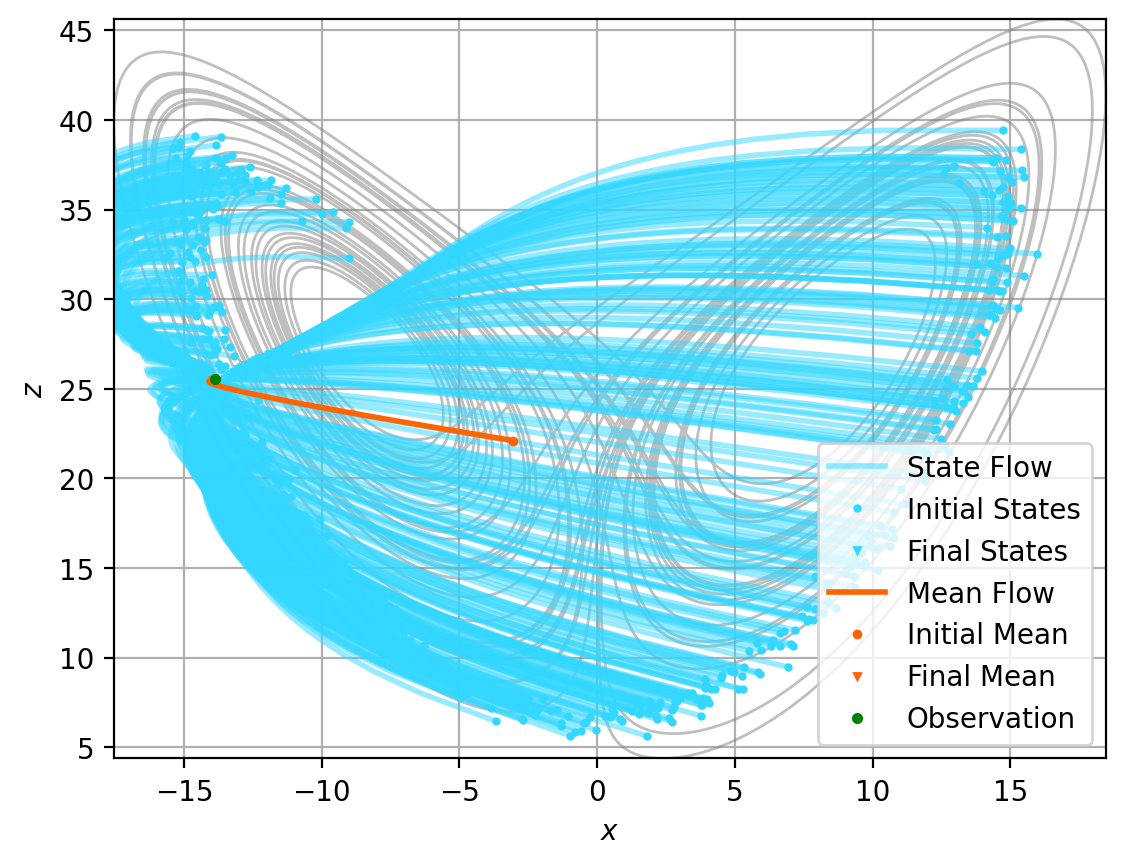
\includegraphics[width=\linewidth]{figures/flow_0_state_0_state_2_signal_background.png}
        \caption{Particle flow in the $q_1$--$q_3$ plane.}
        \label{fig:lorenz_63_propagation_xz}
    \end{subfigure}
    \caption{Lorenz 1963 prior and posterior samples. Courtesy of Prof. Beeson~\cite{beeson2024bayesflow}.}
    \label{fig:lorenz_63_propagation}
\end{figure}

Figure~\ref{fig:lorenz_63_propagation_xy} shows a slice of the three-dimensional model in the $q_1$--$q_2$ plane, whereas Figure~\ref{fig:lorenz_63_propagation_xz} shows a slice in the $q_1$--$q_3$ plane. For our experiment, we treat the three-dimensional initial state samples (blue dots) as the unmapped particle ensemble $\{x^{(i)}\}_{i=1}^n$, and the final-state samples (blue triangles) as the target distribution ensemble $\{z^{(i)}\}_{i=1}^n$. Our goal is once again to optimise a transport map $S$ to cast the prior distribution particles $x^{(i)}$ onto the posterior states $z^{(i)}$.

\subsection{Numerical results} \label{subsec:lorenz_numerical_results}

The optimal transport framework is evaluated on the L63 model dataset across two distinct sample regimes to assess algorithmic robustness to sample sparsity. The first experiment, denoted (a), considers a highly sparse ensemble with $n = 20$ particles, while the second, denoted (b), uses a denser ensemble of $n = 200$ particles. The remaining numerical setup is identical to that of the other experiments. In both configurations, the physical dimension is $D = 3$, and the total-degree truncation parameter is set to $J_k + 1 = 2$. The stochastic gradient descent mechanism is replaced by full-batch gradient evaluations, and the learning rate $\eta$ remains constant with a decay rate of $\gamma = 0$. The complete hyperparameter configuration for both experimental regimes is provided in Table~\ref{tab:lorenz_optimisation_parameters}.

\begin{table}[htbp]
    \centering
    \caption{Parameters for the L63 experiments.}
    \begin{tabular}{lccc}
        \toprule
        \textbf{Parameter} & \textbf{Symbol} & \textbf{(a)} & \textbf{(b)} \\
        \midrule
        Random seed & --                            & 42 & 69 \\
        State dimension & $D$                       & 3 & 3 \\
        Hermite degree & $J_k + 1$                  & 2 & 2 \\
        Particle count & $n$                        & 20 & 200 \\
        Mini-batch cardinality & $B$                & 20 & 200 \\
        Outer PGD iterations & $T$                  & 1000 & 1000 \\
        Dykstra budget & $M_{\mathrm{base}}$        & 100 & 100 \\
        Budget scaling exponent & $p$               & 0.67 & 0.67 \\
        Initial learning rate & $\eta^\circ$        & 0.1 & 0.1 \\
        Learning rate decay & $\gamma$              & 0.0 & 0.0 \\
        IHT interval & $K_{\mathrm{IHT}}$           & 100 & 100 \\
        IHT tolerance & $\varepsilon_p$             & 0.01 & 0.01 \\
        Monotonicity tolerance & $\varepsilon_m$    & 1e-12 & 1e-12 \\
        \bottomrule
    \end{tabular}
    \label{tab:lorenz_optimisation_parameters}
\end{table}

Consistent with the experiments in Section~\ref{subsec:gvm_numerical_results}, the empirical data are normalised prior to the initiation of the projected gradient descent framework to prevent weight degeneracy. The unmapped prior particles $x^{(i)}$ and the target standard normal mapped particles $z^{(i)}$ are whitened to achieve zero mean and unit variance. Upon completion of the outer learning loop at iteration $T-1$, the resulting KR map evaluations are de-whitened to restore the physical dimensions of the geophysical state space.

Results for experiments (a) and (b) are presented in Figure~\ref{fig:lorenz_shear_final} on the top (\ref{fig:lorenz_shear_final_low_particle_count}), and bottom (\ref{fig:lorenz_shear_final_high_particle_count}) figures, respectively. These results are visualised in the $q_1$--$q_2$ plane.

\begin{figure}[htbp]
    \centering
    \begin{subfigure}[t]{\linewidth}
        \centering
        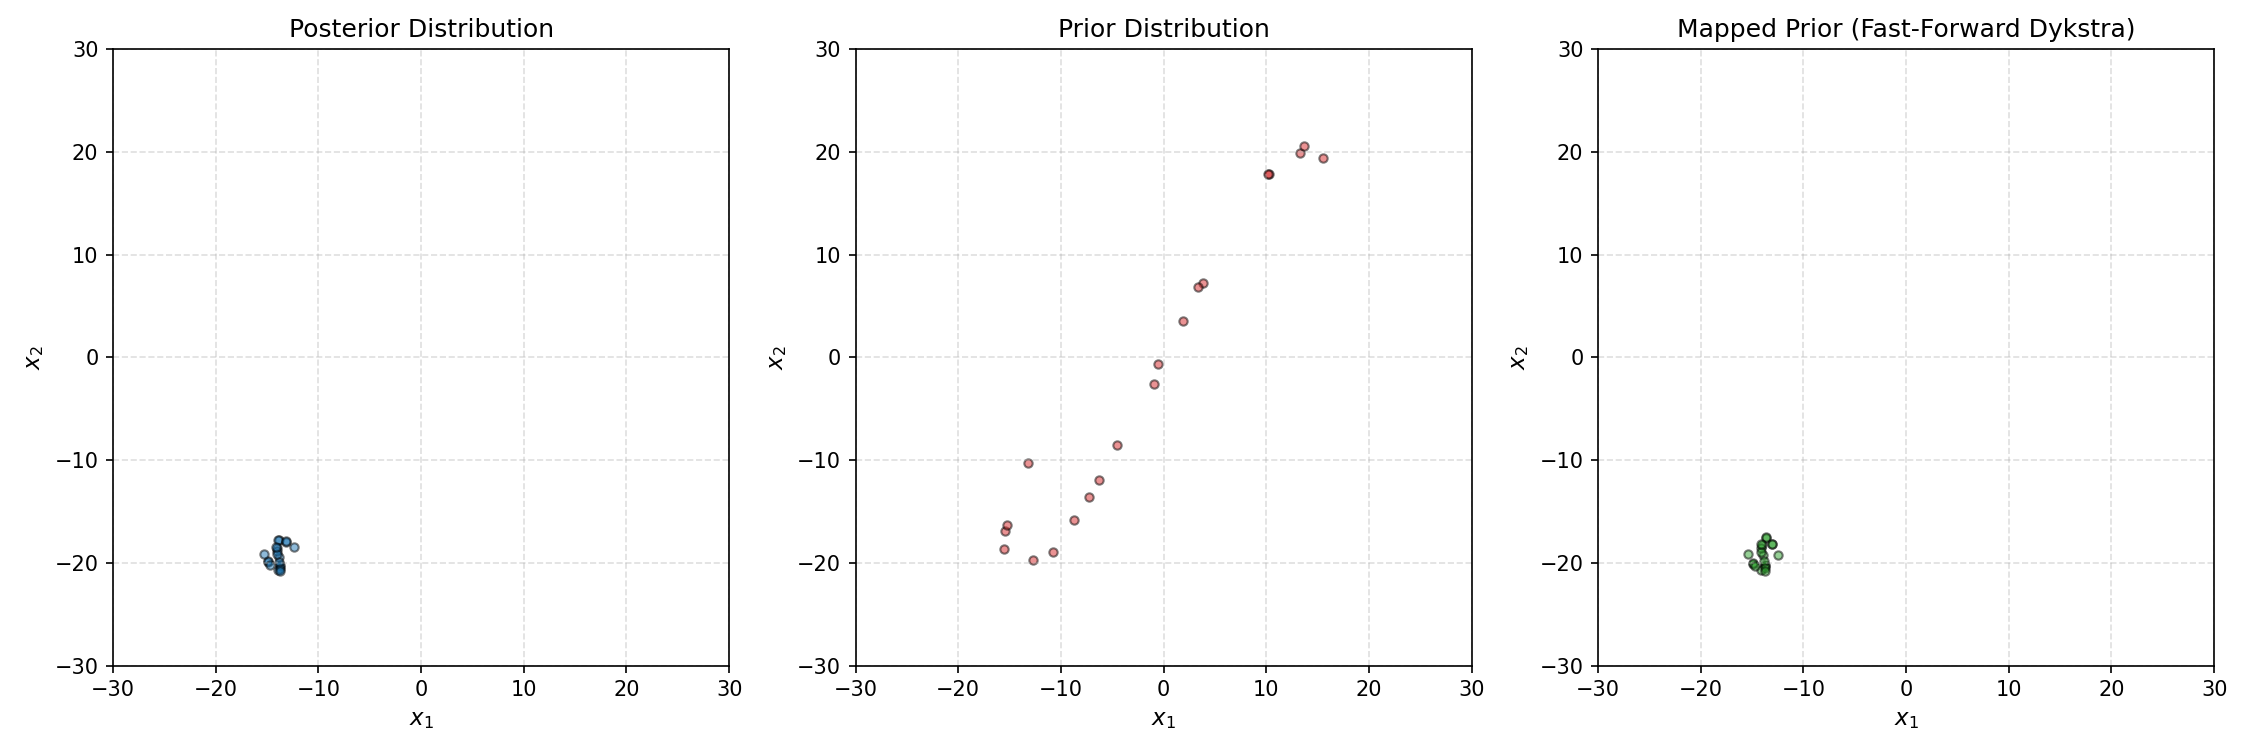
\includegraphics[width=\linewidth]{figures/kr3d_distribution_fast_SEED=42_M=20_D=2_SGD=None_PGDITERS=1,000_DYKSTRA_ITERS=10_10_L1=0.0_LR=1e-01_0e+00_IHT=100.png}
        \caption{Reconstruction with a sparse particle ensemble (\texttt{SEED} $=42$, $n = 20$).}
        \label{fig:lorenz_shear_final_low_particle_count}
    \end{subfigure}

    \vspace{0.5em}

    \begin{subfigure}[t]{\linewidth}
        \centering
        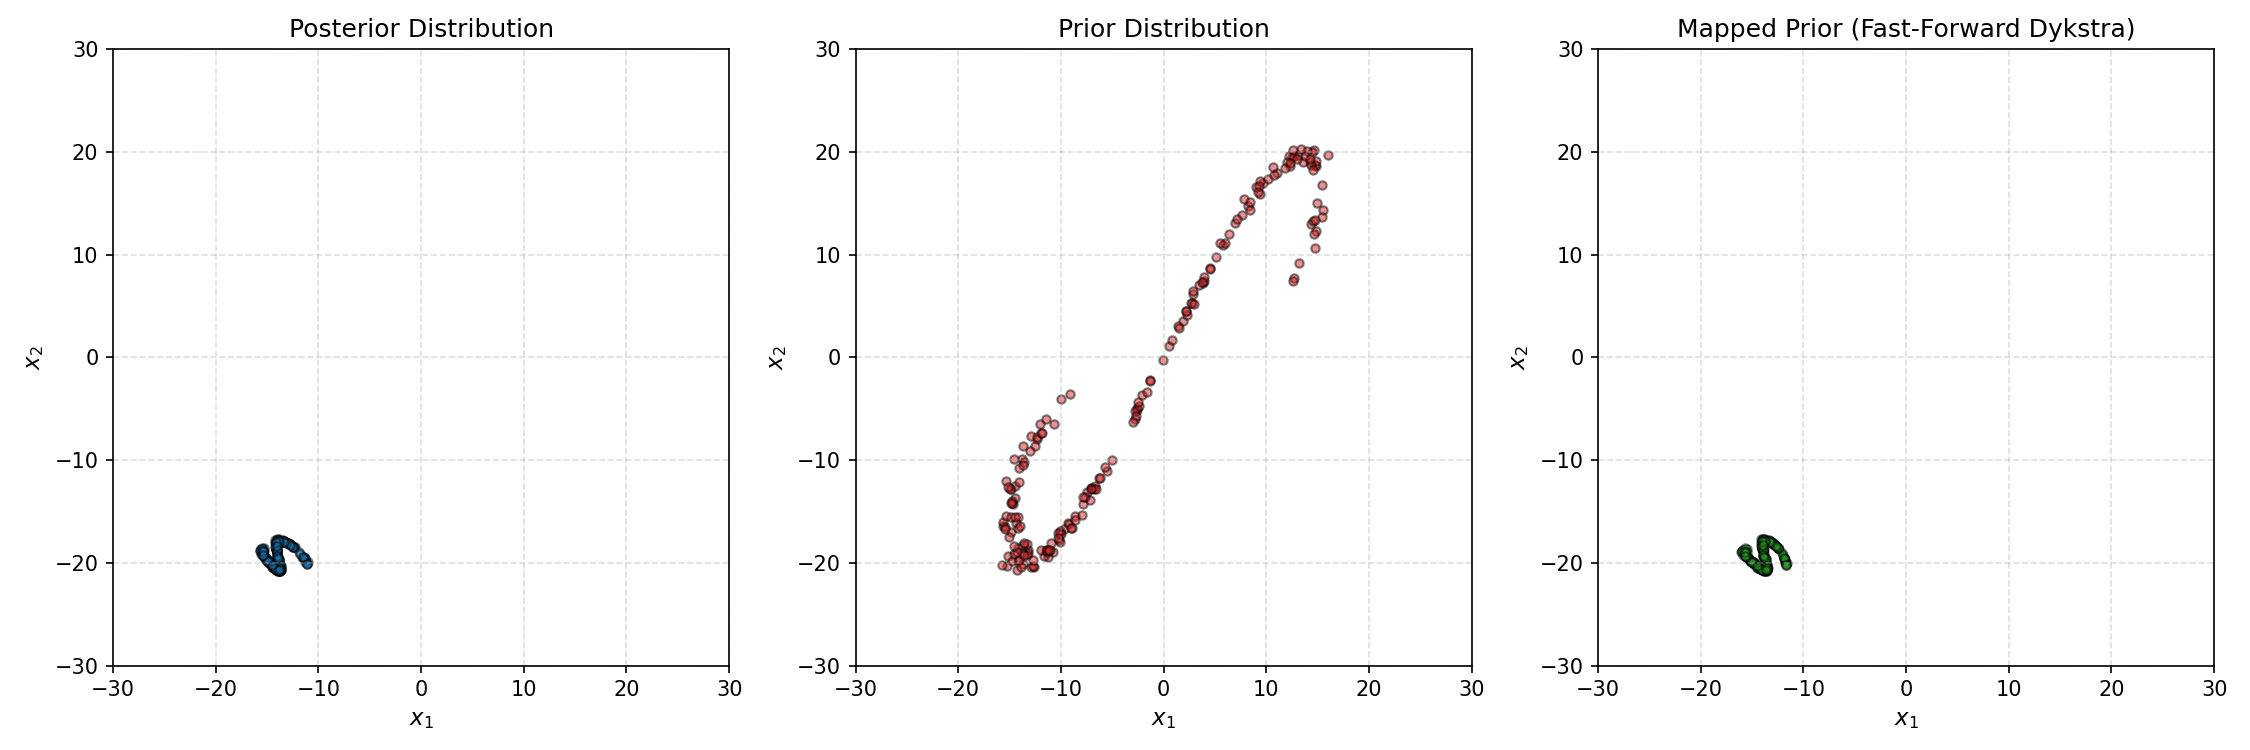
\includegraphics[width=\linewidth]{figures/kr3d_distribution_fast_SEED=69_M=200_D=2_SGD=None_PGDITERS=1,000_DYKSTRA_ITERS=1_10_L1=0.0_LR=1e-01_0e+00_IHT=100.png}
        \caption{Reconstruction with a dense particle ensemble (\texttt{SEED} $=69$, $n = 200$).}
        \label{fig:lorenz_shear_final_high_particle_count}
    \end{subfigure}

    \caption{Optimal transport results for the L63 system.}
    \label{fig:lorenz_shear_final}
\end{figure}

Table~\ref{tab:lorenz_runtime_results} presents the computational runtimes for each configuration. Optimisation of the L63 system dataset maps resulted in reduced execution times relative to previous experiments. This computational efficiency is likely attributable to the lower order of the required transport map.

\begin{table}[htbp]
    \centering
    \caption{Runtimes for the L63 experiments.}
    \label{tab:lorenz_runtime_results}
    \begin{tabular}{@{}lccccc@{}}
        & & \multicolumn{4}{c}{Runtime (s)} \\
        \cmidrule(l){3-6}
        Experiment & Seed & $S^1$ & $S^2$ & $S^3$ & Total \\
        \midrule
        (a) & 42 & 1.14 & 1.19 & 1.27 & 3.60 \\
        (b) & 69 & 2.63 & 2.69 & 2.76 & 8.08 \\
        \bottomrule
    \end{tabular}
\end{table}

Progress videos of the optimised maps for a varying number of outer PGD iterations are made available at:

\begin{center}
    \href{https://drive.google.com/drive/folders/1FEkJWo6-cSvWa-dAoq2DXf_d0Pf9xZye?usp=sharing}{https://drive.google.com/drive/folders/animation\_videos}.
\end{center}

The empirical results from the L63 system demonstrate the generalisability of the optimal transport framework beyond synthetic and aerospace applications. Reconstruction of the KR map to transport the prior forecast measure onto the analysis posterior enables the methodology to circumvent the numerical stiffness associated with traditional observation-flow integration. These findings indicate that addressing the theoretical stalling phenomenon within the foundational projection algorithm produces a robust computational pipeline capable of managing non-linear data assimilation tasks across a range of chaotic systems.